\section{Development}

\subsection*{3.1 Peripherals integration}

The peripherals automation routine was already developed by another student. 
In order to continue the research I took some time to understand the physical concept 
behind EHDA experiments and the project knowledge.

I made upgrades in the routine to include the high speed camera with a hardware triggering routine using an
arduino microcontroler. This will be usefull to validate the further classification of the spray dynamics.


\subsection*{3.2 Experiment tests}

Initial tests were made to verify the setup assembly and the automation routine integration. 
In this step I could unterstand in practise how electrospray works.

I noticed that we need a large set of variables in the range to produce the desired dynamics of electrospray, which most of the time is cone-jet mode.
Those variables can be the liquid properties such as surface tension, dielectric constant, viscosity, density, electrical conductivity and vacuum permitivity.
And also physical variables such as flowrate, system impedance, system temperature, system humidity, nozzle to plate distance, nozzle dimensions and applied voltage.

The instruments used in the setup are:

  - High Voltage Power Supply (FUG)

  - Oscilloscope TiePie WS6 DIFF

  - Humidity and Temperature sensor - DHT11

  - High Speed Camera - Photron fastcam mini

  - Syringe pump

  - Arduino Uno for hardware triggering camera and DHT11 interface


\subsection*{3.3 Data Analysis}

According to Sjaaks paper \emph{A Generic Electrospray Classification}\cite*{Sjaaks} we can classify the spray modes using
only the current data measured by the oscilloscope. With the relations between the statistical values of mean, standart deviation and median of the signal
we can classify if it's in dripping or cone-jet dynamics. In the figure below we can see the current data acquired from one experiment and also the statistical levels
above. Each sample takes a frame window of 0.5s of current data and then classifies it.

For each sample color the algorithm classifies:

  - green: dripping mode

  - blue: intermittent mode

  - red: Cone-jet mode

  - purple: corona spark mode


\begin{figure}[H]
    \center
    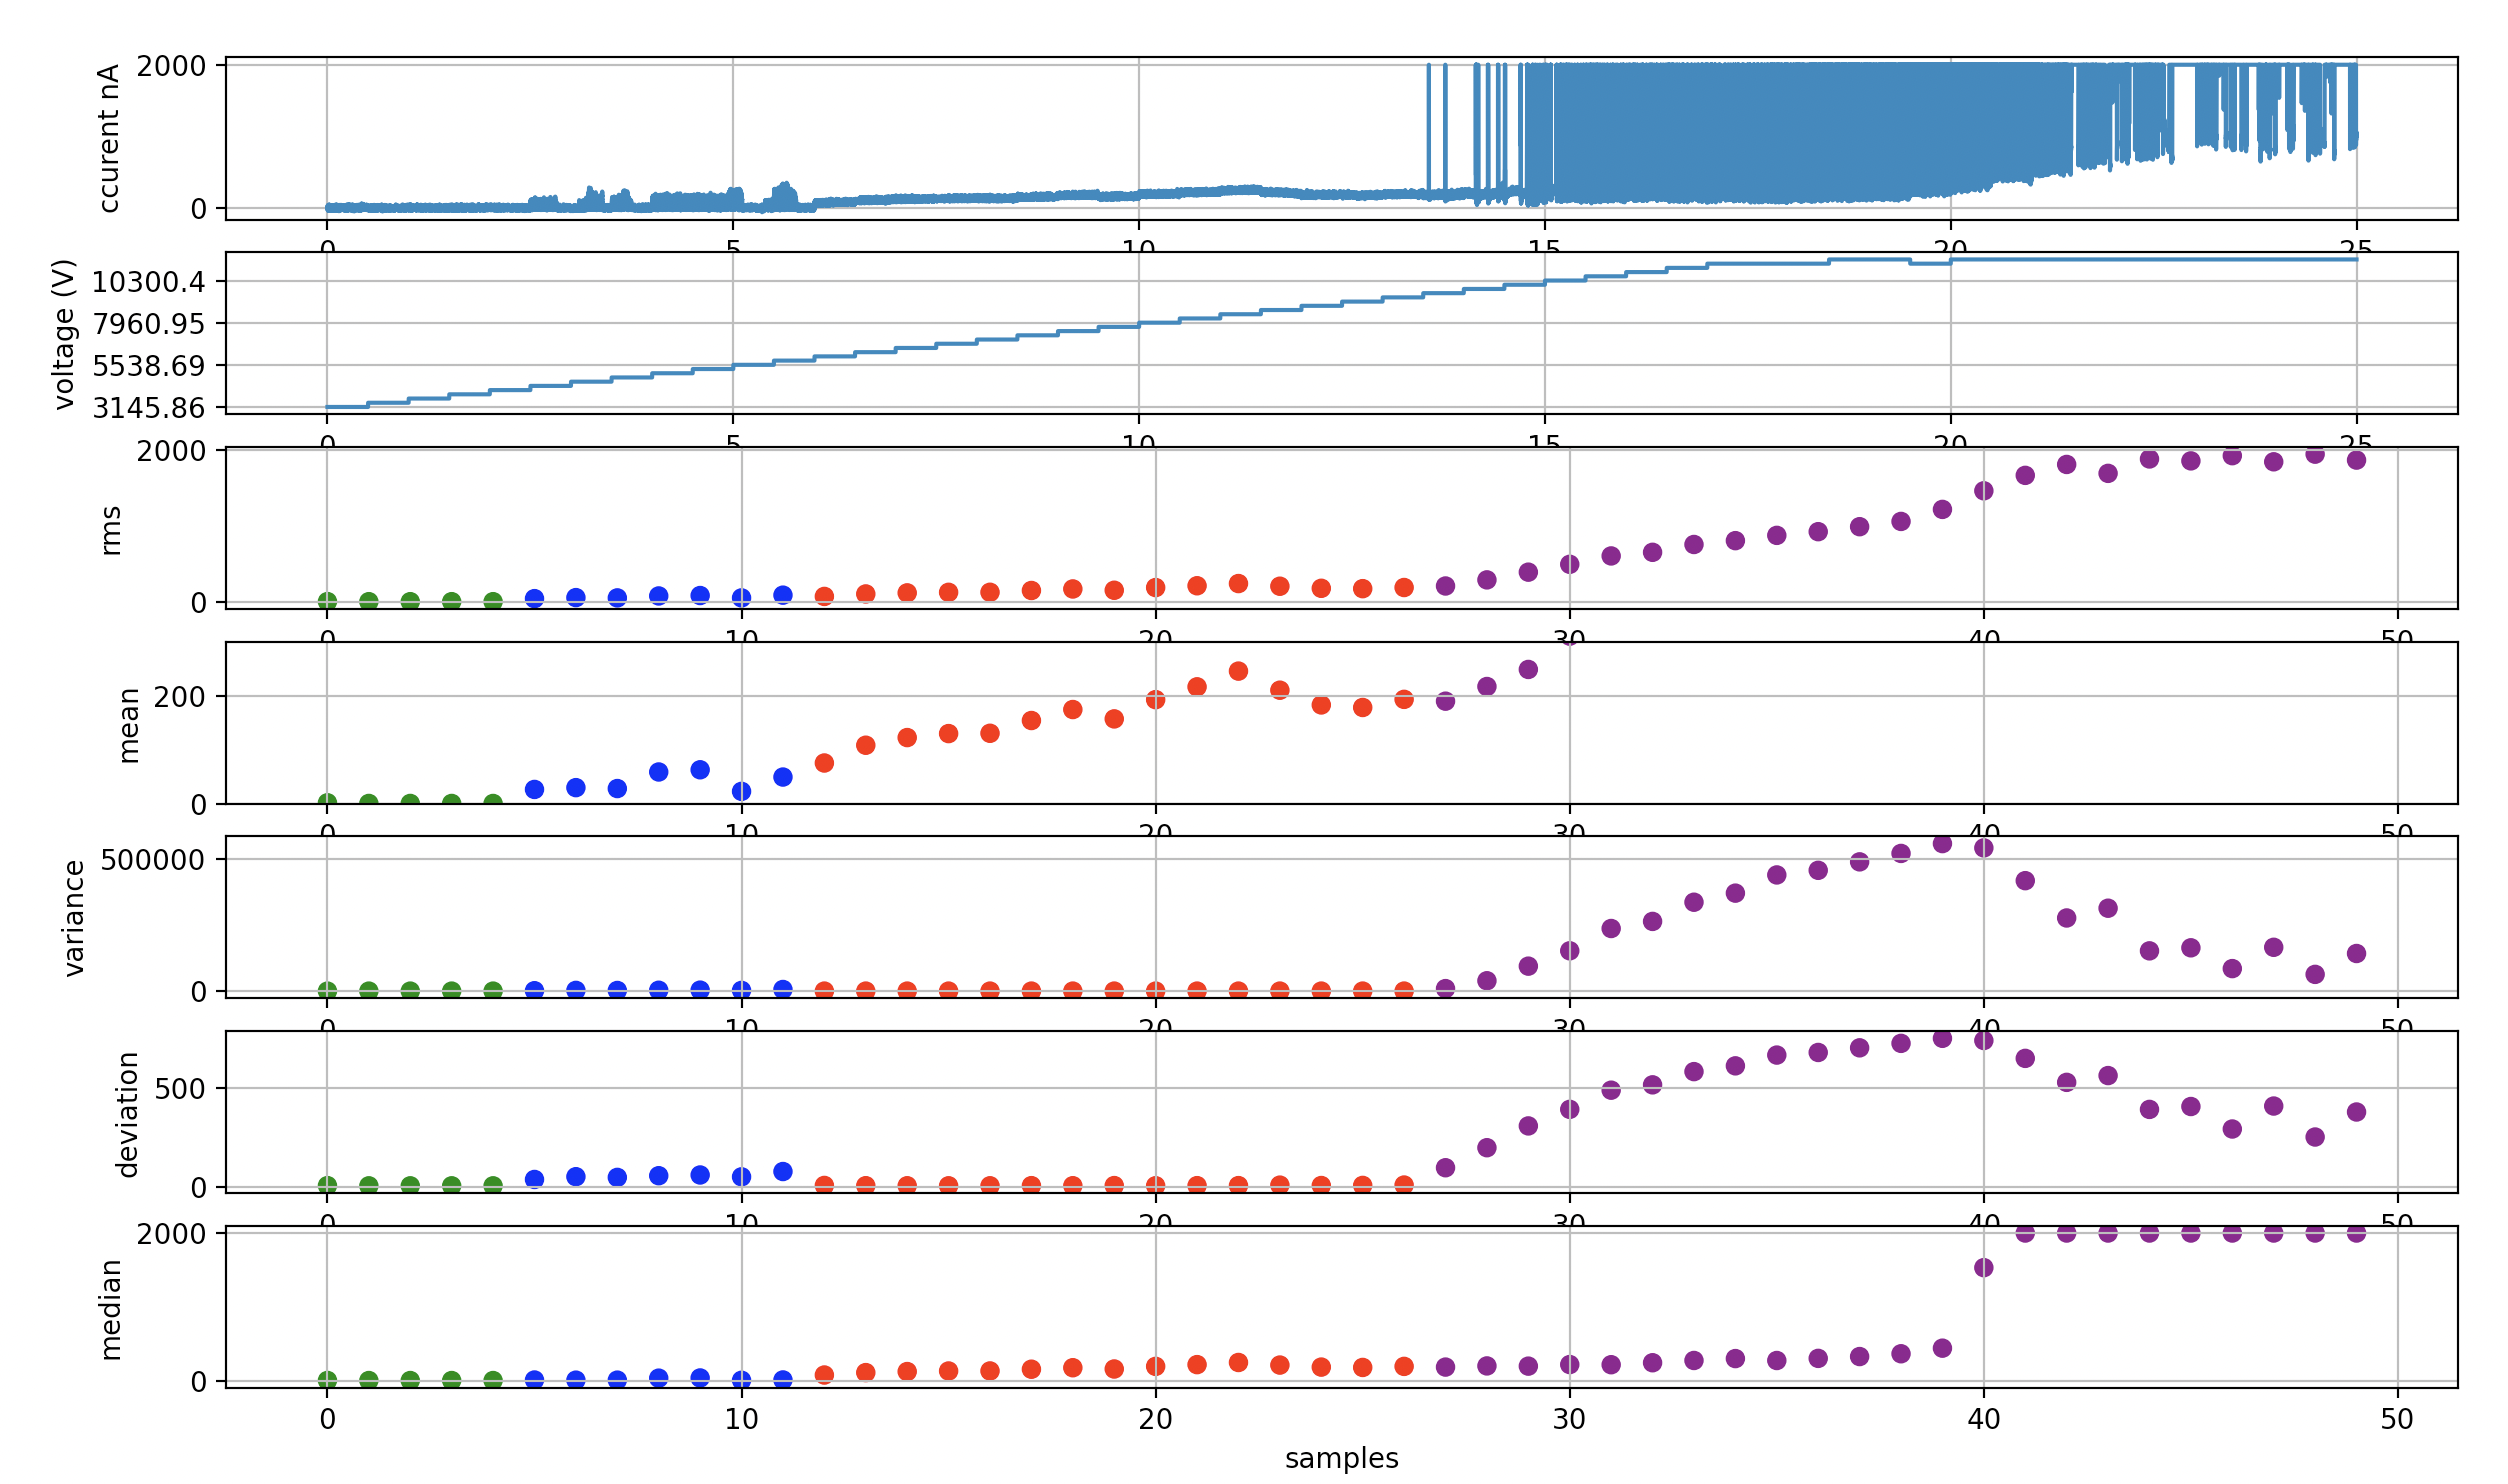
\includegraphics[width=12cm]{images/exp_data.png}
    \label{img2}
    \caption{Data Analysis}
\end{figure}


